\subsection{Entity-Relationship Schema}

    \begin{center}
        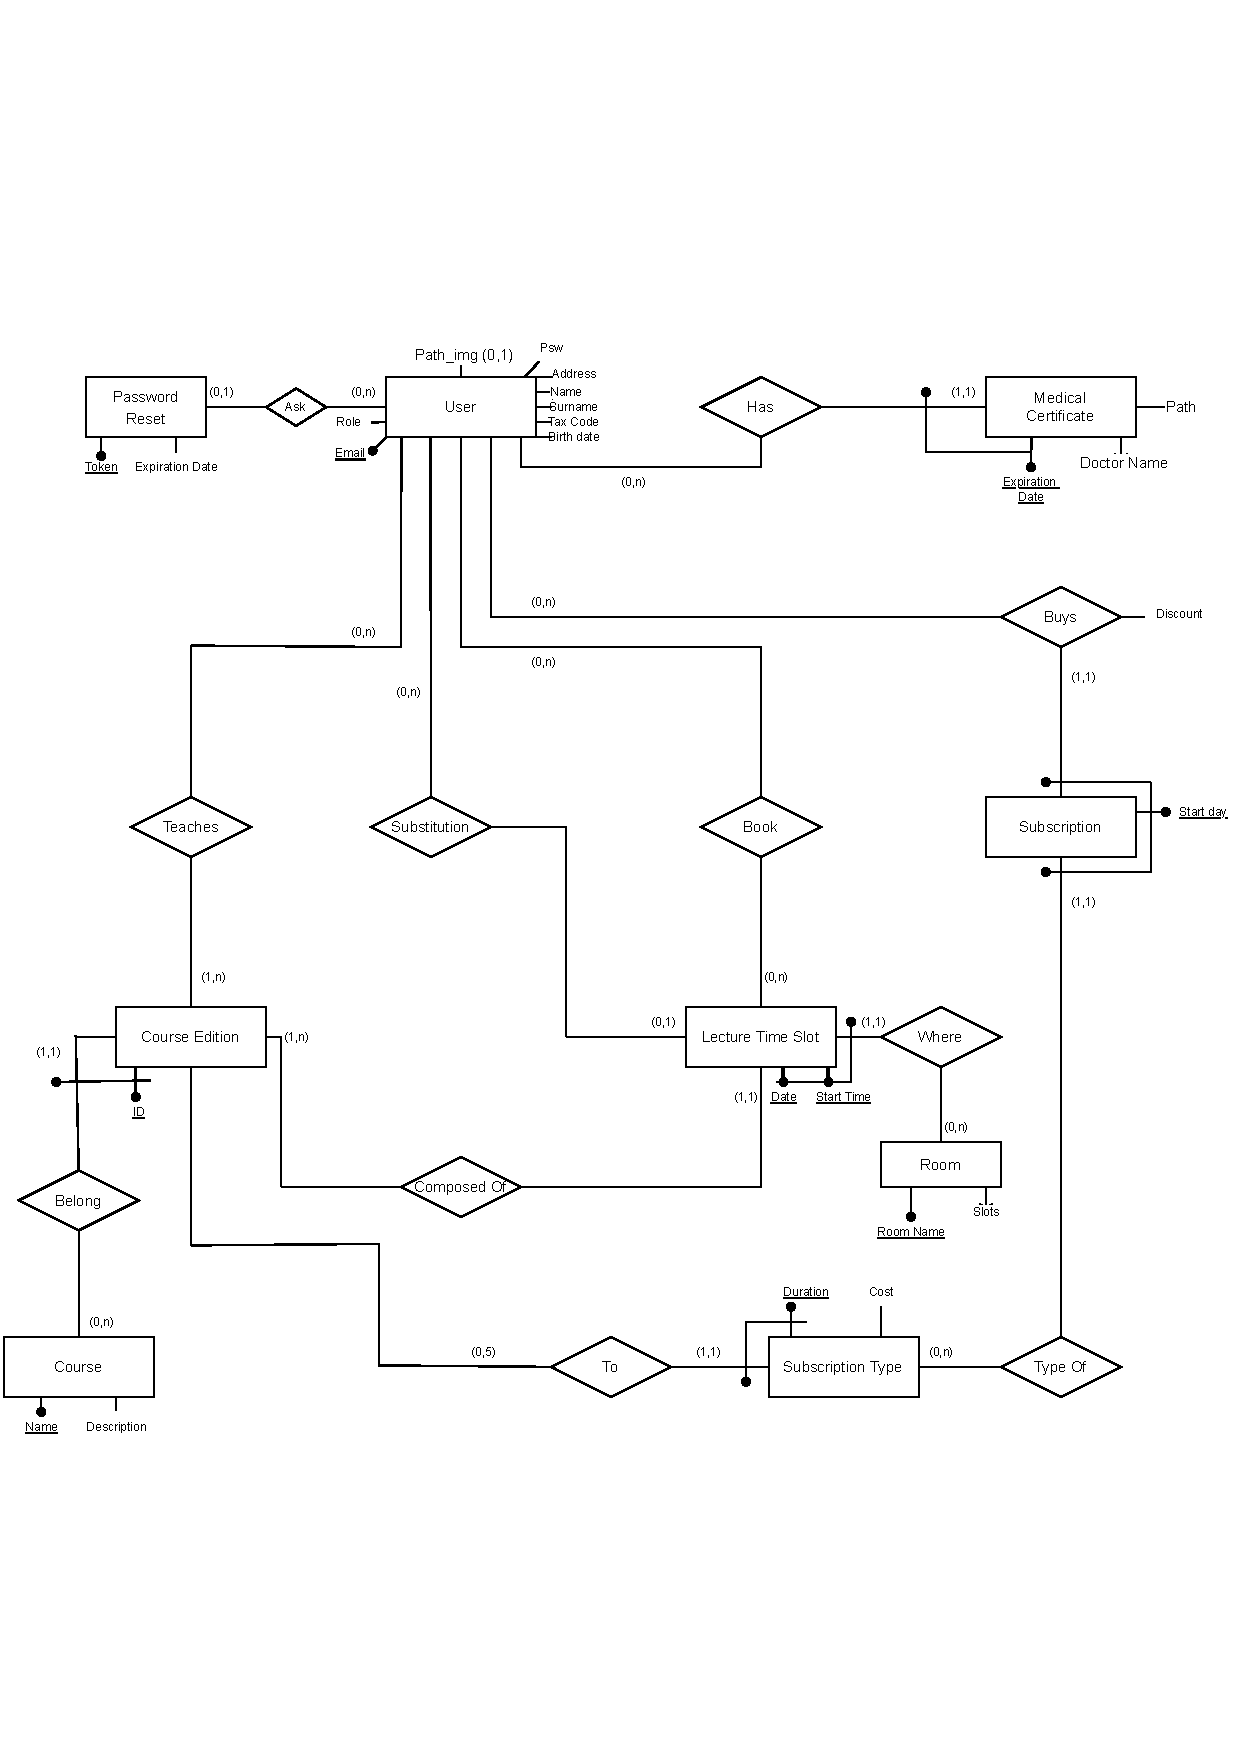
\includegraphics[width=0.9\textwidth]{resources/ER_restructured_v2.pdf}
        % this isn't finished yet
    \end{center}

    The entity-relationship contains 9 main entities:
    \begin{itemize}
        \item 
        \textbf{User}: each user of the application is identified by an \textit{Email} (type of VARCHAR). 
    	For each user we also save their \textit{Name}, \textit{Surname}, \textit{Address}, \textit{Telephone} and \textit{Avatar Path} (for users's Profile image) as VARCHAR fields (Optional). We also save user's \textit{Birthday} (of type DATE). For each users we define
        one or more Roles (Indicated in the role attribute). The roles are:
        \begin{itemize}
			\item Trainer: They held courses at the gym 
			\item Trainee: Users which subscribes in order to partecipate to courses
			\item Secretary: Users that managed course subscriptions and in charge to sign presence
        \end{itemize}
    	
    	\item \textbf{Course}: The gym has different courses and each of them is uniquely identified by \textit{Name} (type of VARCHAR). Each course also has and additional attribute \textit{Description} of type TEXT.
    	
    	\item \textbf{Course Edition}: Each course may have many course editions. Each course eddition is identified by the \textit{ID}(of type SERIAL), and \textit{CourseName}(which is the identifier of the entity Course).
    	
    	\item \textbf{Room}: Lessons of each course are held in a Room which is identified by its \textit{Name} (type of VARCHAR). Each room has an attribute, \textit{Slots}(of type INTEGER), for the capacity of the Room.
    	
    	\item \textbf{Lecture Time Slot}: Each Course Edition is composed of severls Lectures Time Slot. Each Lecture Time Slot is identified by three fields : \textit{Date}(of type Date)), \textit{Start Time}(of type Time) and \textit{Room}(of type Room). Each Lecture Time Slot has a fixed duration of 2 hours.
    	
    	\item \textbf{Subscription Type}: Each Course Edition can have at most 5 types of Subscription Type(Dayly, Monthly, Quaterly, Half-Yearly, Yearly). Each Subscription Type, is identified by two fields : \textit{Duration}(of type INTEGER that indicates how many days the subscription type last) and \textit{Course Edition}(of type Course Edition). In addition, Subscription Type has also a field \textit{Cost}(of type DECIMAL) to express the cost of a Subscription Type for different Durations and for different Course Editions.
    	
    	\item \textbf{Subscription}: A Trainee can have several Subscription. Every subscription is identified by \textit{Start Day}(of type Date), \textit{Trainee}(of type User) and \textit{Subscription Type}(of type Subscription Type). When a trainee buys a Subscription, if it was made in a particular day of the year (i.e. during the black friday week), he or she can have a discount applied to it.
    	
    	\item \textbf{Password Reset}: Additional entity to allow users to reset their password (a User can change multiple times its password). It's identified by the \textit{Token} (type of VARCHAR) and has another field called \textit{Expiration Date}(type of TIMESTAMP).
        
        \item \textbf{Medical Certificate}: Entity used to store the medical certificate of a given user. It's identified by the \textit{Trainee}(of type User). It also has another field : \textit{Expiring Date}(of type of DATE). It has two additional attributes: \textit{Doctor Name} (type of VARCHAR) and \textit{Path} (type of TEXT).
        
        \item \textbf{Type of Roles}: Entity used to store the roles available for a User.
        
        \item \textbf{Email Confermation}: Additional entity to allow a User to confirm its registration after he has done it.
	
    \end{itemize}